\section{Afstand}
\label{DatabehandlingRAfstand}
%
I dette afsnit analyseres resultaterne med udgangspunkt i de tre forskellige afstande robotten havde til testpersonerne i testen. De forskellige afstande fremgår af \autoref{tab:RDistance}, hvor antallet af testpersoner ligeledes er opgivet. 

Det undersøges, hvordan robottens afstand påvirker de rejsendes oplevelse af robotten ved at undersøge, hvordan resultaterne ændrer sig afhængigt af de tre forskellige afstande. Det er et \textit{Between-subject} design, da hver testperson kun har oplevet robotten i én af afstandende og svaret ud fra denne.
%
\begin{table}[H]
\centering
\begin{tabular}{c|c}
Afstand & Antal testpersoner \\ \hline
Tæt på (1) & 7    \\ \hline
Tilpas (2) & 28    \\ \hline
Langt fra (3) & 8     \\ 
\end{tabular}
\caption{Oversigt over antallet af testpersoner til hver af de tre afstande robotten havde.}
\label{tab:RDistance}
\end{table}
\noindent
%
Ud fra \textit{Scree}-plottet på \autoref{fig:Distance-Scree} fremgår det at cirka 80 \& af variansen kan forklares ud fra den første \textit{Principal Component} (PC) og 100 \% af variansen kan forklares ud fra to PCs. 
%
\begin{figure}[H]
\centering
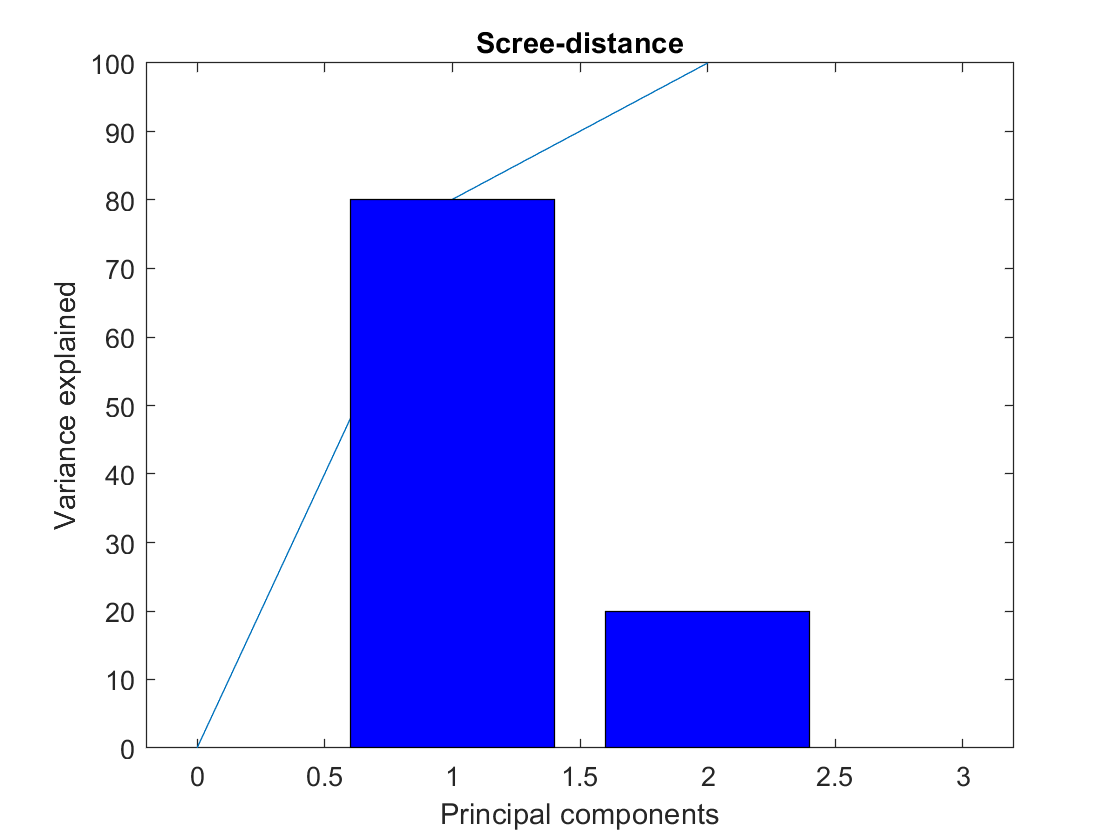
\includegraphics[width=\textwidth]{Figure/DatabehandlingSkalaer/PCAfigures/Distance-Scree.png}
\caption{\textit{Scree}-plot, hvorpå sammenhængen mellem antallet af \textit{Principal Components} og \textit{Variance Explained [\%]} fremgår: PC1 (80.1\%), PC2 (19.9\%).}
\label{fig:Distance-Scree}
\end{figure}
\noindent
%
Ud fra \textit{Score}-plottet på \autoref{fig:Distance-Score} fremgår det, at der generelt er en del spredning mellem resultaterne ud fra de tre forskellige afstande, hvilket foreskriver at de tre afstande ikke umiddelbart har ens karakteristikas.
%
\begin{figure}[H]
\centering
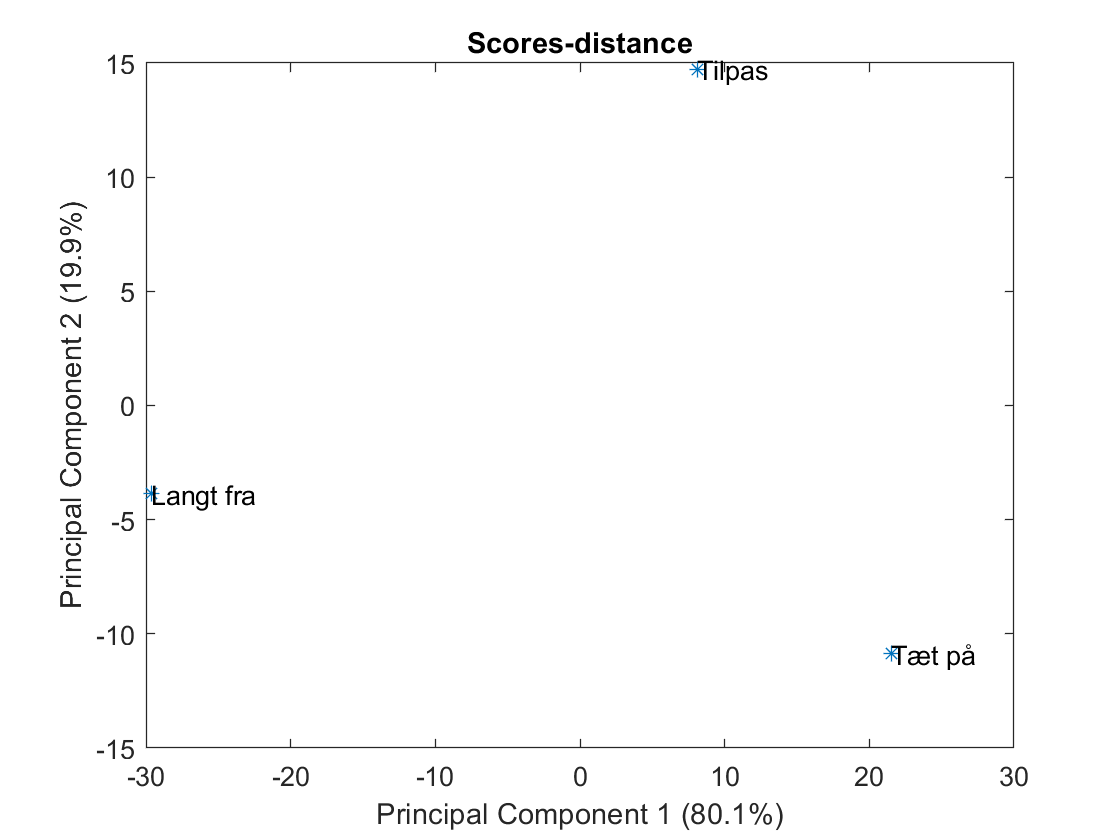
\includegraphics[width=\textwidth]{Figure/DatabehandlingSkalaer/PCAfigures/Distance-Scores}
\caption{\textit{Score}-plot for PC1 og PC2 i forhold til de tre afstande robotten holder til testpersonerne.}
\label{fig:Distance-Score}
\end{figure}
\noindent
%
I henhold til de tre afstande tyder det ikke på, at afstanden \textit{Langt fra} påvirkes særlig meget af nogen af parametrene, da ingen \textit{loadings} peger direkte mod eller er tæt på denne afstand, jævnfør \autoref{fig:Distance-Biplot}. Det tyder derimod mod på, at afstanden \textit{Tilpas} hovedsageligt er domineret af SQ2, SQ10 og SQ22, hvor afstanden \textit{Tæt på} primært domineres af SQ1 og tildels SQ14.     

Ud fra \textit{Bi}-plottet på \autoref{fig:Distance-Biplot}, hvorpå \textit{loadings} og \textit{scores} for hver parameter er præsenteret, fremgår det at SQ1, omhandlende skærmens reaktion, og SQ15, vedrørende hvor overraskede testpersonerne blev ved robottens henvendelse, bidrager mest til PC1. Hvor for PC2 er det SQ10, vedrørende hvor tryg testpersonerne følte sig ved robotten, som har det største bidrag. Derudover tyder det på at både SQ11, vedrørende hvorvidt robotten gjorde testpersonerne forskrækket, og SQ17, vedrørende robottens elegance, kun beskriver en lille del af variansen, hvorfor det ikke giver mening at kommentere på, hvordan de indbyrdes ligger, medmindre de indgår i en korrelation med en mere betydende parameter.   
%
\begin{figure}[H]
\centering
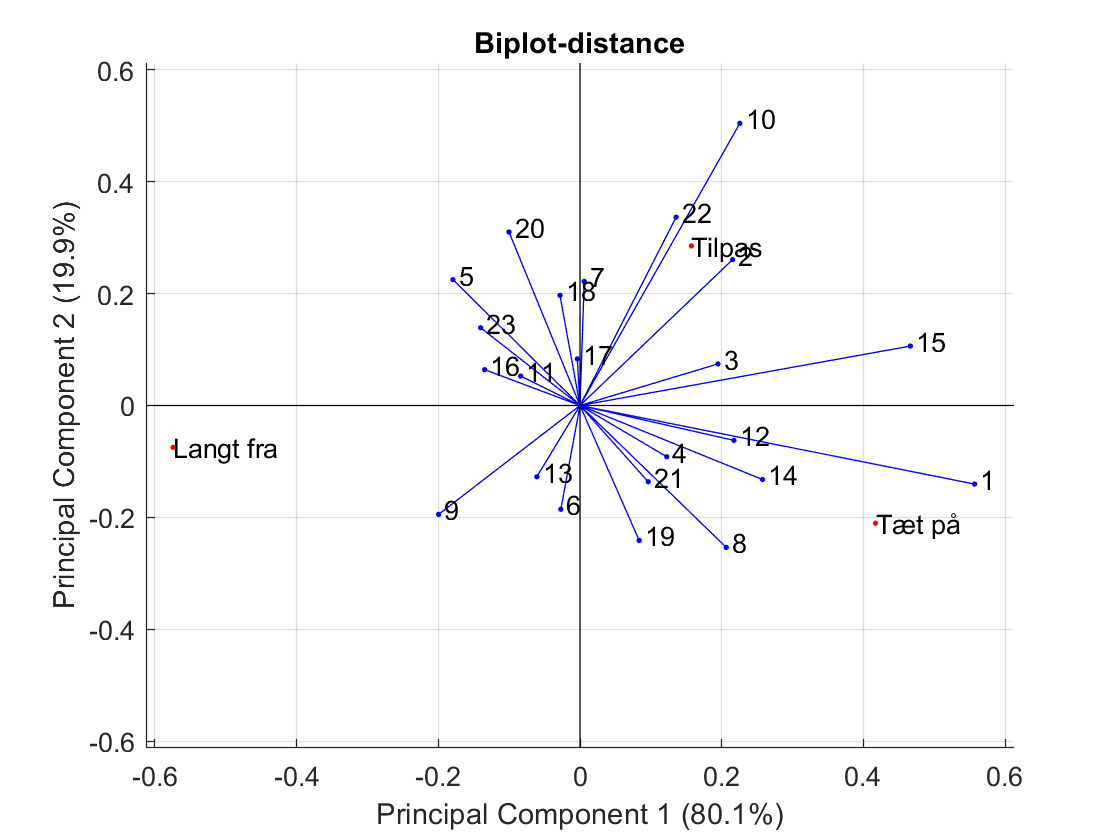
\includegraphics[width=\textwidth]{Figure/DatabehandlingSkalaer/PCAfigures/Distance-Biplot.png}
\caption{\textit{Bi}-plot med både \textit{loadings} (angivet med blå) og \textit{scores} (angivet med rød) fremgår i forhold til robottens afstand.}
\label{fig:Distance-Biplot}
\end{figure}
\noindent
%
Ud fra \autoref{fig:Distance-Biplot} fremgår det, at SQ1, vedrørende skærmens reaktion, og SQ12, vedrørende hvor godt testpersonen kan lide at blive betjent af robotten, ligger tæt på hinanden, hvorfor de er korrelerede. Korrelationen skyldes ikke at de to parametre måler det samme, men formentlig påvirker hinanden, så når skærmen reagerer dårligt så vil det have en negativ effekt på hvor godt testpersonerne kan lide at blive betjent af robotten. Da det forventes at den færdigudviklede robot vil have en skærm, hvis reaktionsevne er væsentligt bedre end hvad der har været tilfældet i projektet, vurderes det at SQ1 formentlig kan være redundant. 

Lignende gør sig gældende for SQ10, vedrørende hvor tryg testpersonerne følte sig ved robotten, og SQ22, vedrørende hvor sjov robotten er. Det giver mening, at de to parametre korrelerer da det antages, at hvis testpersonerne føler sig utrygge så vil de formentlig heller ikke opleve robotten som værende sjov. Det vurderes derfor, at de to parametre formentlig ikke måler det samme. For SQ8, vedrørende hvorvidt testpersonerne føler, at robotten kan hjælpe dem, og SQ21, vedrørende hvor anmassende robotten er, forekommer samme tendens; at de to parametre er positivt korreleret. Denne korrelation skyldes formentlig ikke, at de to parametre måler det samme, da anmassende også kan vedrører at robotten kommer for tæt på, hvilket afspejles ved den negative korrelation med SQ5, vedrørende robottens afstand. \blankline
%
Udover de positive korrelationer forekommer der ligeledes negative korrelationer, hvilket blandt andet gør sig gældende for SQ2, vedrørende robottens bevægelser, og SQ9, vedrørende hvorvidt testpersonerne synes, at robotten stod i vejen. Lignende er gældende for den positive korrelation mellem SQ10 og SQ22, som har en negativ korrelation med SQ13, vedrørende hvorvidt testpersonerne følte, at robotten fulgte dem hen til det valgte sted. Den negative korrelation, der forekommer mellem SQ10 og SQ13 blev fundet som værende positiv i foregående analyse omkring højden. Ydermere forekommer der negativ korrelation mellem SQ14, vedrørende hvor personlig robottens hjælp opleves, og SQ16, vedrørende hvor irriterende robotten opleves. 

Derudover tyder det på, at der er en negativ korrelation mellem SQ19, vedrørende hvor sød robotten opleves, og SQ20, vedrørende hvor sej robotten opleves.\blankline
%
Hver \textit{loading} angiver hvor meget variation hver parameter bidrager med i forhold til den specifikke PC. I \autoref{tab:LoadingsAfstand} fremgår samtlige \textit{loadings} for hver parameter til hver PC. 
%
\begin{table}[H]
\centering
\begin{tabular}{c|c|c}
    & PC1 (80.1\%)    & PC2 (19.9\%)    \\ \hline
SQ1  & \textbf{0.5567} & -0.1405         \\ \hline
SQ2  & 0.2152          & 0.2608          \\ \hline
SQ3  & 0.1945          & 0.0744          \\ \hline
SQ4  & 0.1224          & -0.0917         \\ \hline
SQ5  & -0.1793         & 0.2251          \\ \hline
SQ6  & -0.0271         & -0.1856         \\ \hline
SQ7  & 0.0059          & 0.2217          \\ \hline
SQ8  & 0.2064          & -0.2537         \\ \hline
SQ9  & -0.1995         & -0.1946         \\ \hline
SQ10 & 0.2255          & \textbf{0.5045} \\ \hline
SQ11 & -0.0838         & 0.0526          \\ \hline
SQ12 & 0.2171          & -0.0623         \\ \hline
SQ13 & -0.0609         & -0.1274         \\ \hline
SQ14 & 0.2575          & -0.1323         \\ \hline
SQ15 & 0.4661          & 0.1062          \\ \hline
SQ16 & -0.1346         & 0.0641          \\ \hline
SQ17 & -0.0038         & 0.0834          \\ \hline
SQ18 & -0.0283         & 0.1969          \\ \hline
SQ19 & 0.0834          & -0.2412         \\ \hline
SQ20 & -0.1002         & 0.3102          \\ \hline
SQ21 & 0.0962          & -0.1363         \\ \hline
SQ22 & 0.1356          & 0.3367          \\ \hline
SQ23 & -0.1403         & 0.1390         
\end{tabular}
\caption{Oversigt over \textit{loadings} til de to PCs, for hver PC fremhæves den mest betydende parameter. \textit{SQ} angiver skala spørgsmålet.}
\label{tab:LoadingsAfstand}
\end{table}
\noindent
%

\subsection{Tendenser i forhold til robottens afstand}
\label{DatabehandlingAfstandTendenser}
%
Da det ikke har været muligt at kontrollere afstanden mellem robotten og testpersonerne, dels fordi det ikke har været muligt at måle en decideret afstand og fordi det kan ændre sig løbende i interaktionen, er det begrænset hvad der kan udledes af tendenser, hvorfor de ikke fremgår her. Dog forefindes samtlige grafer i \fullref{ElektroniskBilagTendenser}. Det har dog været muligt, at finde en tendens til at testpersonerne bliver mere overrasket når robotten er tæt på end når den er langt fra, jævnfør \autoref{fig:TendensDistanceSQ15}. På figuren henviser afstand 1 til tæt på, afstand 2 til tilpas og afstand 3 til langt fra. 
%
\begin{figure}[H]
\centering
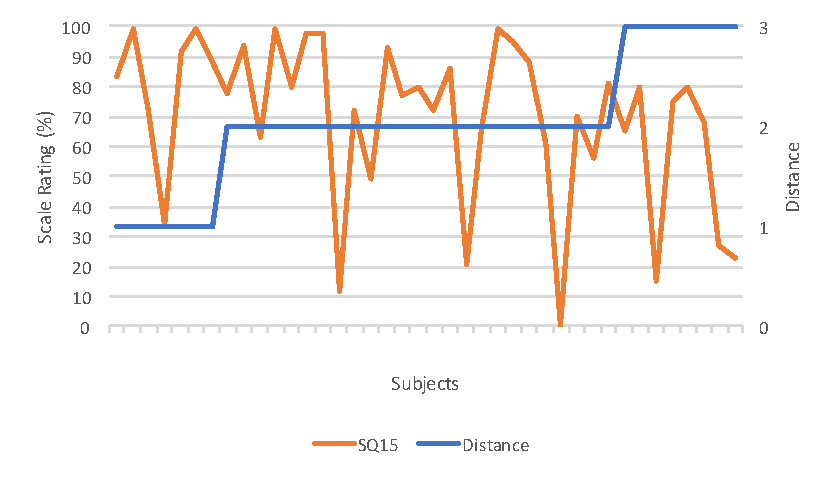
\includegraphics[width=\textwidth]{Figure/DatabehandlingSkalaer/TendensHeight/DistanceSQ15}
\caption{Sammenhæng mellem robottens tre afstande og hvad testpersonerne angiver (\%) på skalaen til SQ15: \textit{Hvor overrasket blev du over robottens henvendelse?}. Denne graf bygger på 40 besvarelser, da der manglede tre. Afstand 1 svarer til at robotten kommer tæt på, afstand 2 til en tilpas afstand og afstand 3 til at robotten stopper for langt fra.}
\label{fig:TendensDistanceSQ15}
\end{figure}
\noindent
%
